\gobbletocpage
\chapter{Prior Work}
\restoretocpage

%\begin{shadequote}
%If I have seen further it is by standing on the shoulders of giants.\par\emph{Isaac Newton}
%\end{shadequote}

%cut out up to we?
\begin{shadequote}
%Bernard of Chartres used to say that
We are like dwarfs on the shoulders of giants, so that we can see more than they, and things at a greater distance, not by virtue of any sharpness of sight on our part, or any physical distinction, but because we are carried high and raised up by their giant size.\par--\emph{John of Salisbury}
\end{shadequote}

\section{Background and Theory}
While the previous chapter summed up the purpose and motivation of developing a theory-based approach to understanding bacterial speciation, this chapter will provide the reader with the prerequisite knowledge necessary to thoroughly understand ES, the improvements described in chapter three, and my experimental designs in chapter four.

\subsection*{Ecotype model of bacterial species}
%An ecotype is defined as a bacterial cluster with individuals that are ecologically similar to one another, so much so that genetic diversity within the ecotype is limited by a cohesive force: periodic selection, genetic drift, or both~\cite{cohan2007systematics}.
We define ecotype here as a phylogenetic group of close relatives that are ecologically interchangeable, in that the members of an ecotype share genetic adaptations to a particular set of habitats, resources, and conditions; also, ecotypes are ecologically distinct from one another.
This definition contrasts to with earlier ecotype concepts, in that the present definition of ecotype implies no other species-like characteristics beyond ecological distinctness~\cite{wiedenbeckHGT}.
By linking species and ecological niche we take advantage of the natural clustering of organisms according to their environmental resources.
Since these clusters are evolving together we do not need to utilize morphological differences and can instead use a molecular approach for demarcation.

%Would I then take this portion out?
Ecotypes have all the dynamic properties of a species: each is a cohesive group, different ecotypes are irreversibly separate because they are out of range of one another's cohesive force, and because recombination is too rare to prevent their adaptive divergence; they are by definition ecologically distinct, which allows them to coexist into the future~\cite{cohan2007systematics}.
They are our fundamental unit of microbial ecosystems.
Efforts to define prokaryotic species according to these properties have differed most profoundly in the forces of cohesion thought to be most important for prokaryotic species~\cite{cohan2008origins}.
ES uses one model in particular to understand ecotype bacterial speciation.

\subsection*{Stable Ecotype model}

\begin{figure}[h!]
% \caption{Three classes of mutation and recombination events that determine ecotype diversity in bacteria. Circles represent different genotypes, and asterisks adaptive mutations. (A) Periodic selection purges diversity. (B) Ecotype formation creates diversity. (C) Extinction events SHOULD I CUT THIS OUT?.(reprinted from \protect\cite{cohan2007systematics})}
 \centering
 \label{fig:StableEvents}
 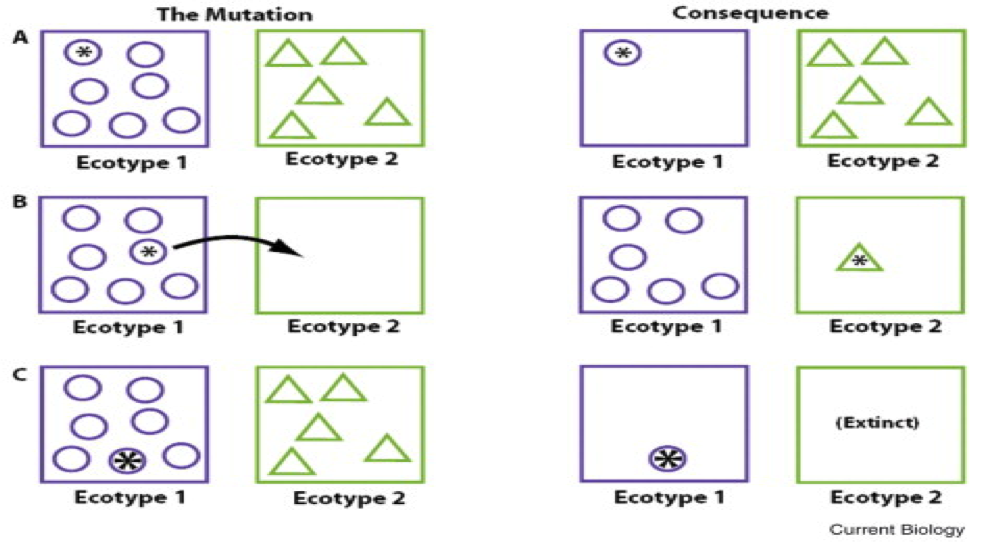
\includegraphics{images/StableEcotypeEvents-CH2}
 \caption[Events predicted by the Stable Ecotype model.]{Three classes of mutation and recombination events that determine ecotype diversity in bacteria. Circles and triangles represent individual organisms, and asterisks adaptive mutations. (A) Periodic selection purges diversity. (B) Ecotype formation creates diversity. (C) Extinction events (reprinted from \protect\cite{cohan2007systematics}).}
 \label{fig:StableEvents}
\end{figure}

In the Stable Ecotype model, ecotypes are created and extinguished at a very low rate, and during an ecotype's long lifetime it is recurrently purged of its diversity by periodic selection events~\cite{cohan2007systematics}.
Ecotypes are formed rarely enough so that each ecotype can accumulate its own set of unique mutations while diversity is purged recurrently, yielding a correspondence between ecotypes and sequence clusters for any gene shared among ecotypes~\cite{cohan2008origins}.
This fact, hinted at earlier, is what allows ES to identify separate ecotypes based on environmental function without knowledge of particular phenotypic mutations.
Diversity quashing events are referred to as periodic selection events (see Figure~\ref{fig:StableEvents}A).
An individual within an ecotype acquires a mutation that improves its fitness within that ecological niche, which results in a diversity purge, due to low recombination rates in bacteria, where other organisms in the ecotype without the adaption become extinct.
Genetic drift is another event that results in diversity purges, however it normally occurs at low rates (except in small sample sizes), thus we will refrain from mentioning it in the future.

%Describes relationship of periodic selection events and ecotype formation event
%I don't think this is correct, double check!!
Early during speciation, a new ecotype's niche may rely on the proportions of resources used and may be vulnerable to extinction by periodic selection caused by an adaptive mutation within the parental ecotype.
However, a single HGT event may transfer the adaptive mutation across ecotypes, and could thereby prevent extinction of one ecotype by another~\cite{cohan2008origins}.
In this case an ecotype formation event occurs (see Figure~\ref{fig:StableEvents}B).
The ecotype-transcending adaptation allowed an ecotype speciation event to occur. In the figure an individual of an ecotype developed an adaptation that went on to colonize a new niche creating a new ecotype.

Now we have an event to account for anagenesis, or accumulation of changes over time along a single lineage, referred to as periodic selection, and cladogenesis, or irreversible splitting of lineages, referred to as ecotype formation.
To complete the dynamics of the Stable Ecotype model, extinction events are also possible (see Figure~\ref{fig:StableEvents}C).
Naturally, an ecotype can go extinct.
Previous work done in the Cohan lab resulted in an algorithm based on the Stable Ecotype model, known as Ecotype Simulation (ES).


\section{The Algorithm}

\begin{SCfigure}
 \caption[Phylogenetic tree representation of typical Stable Ecotype model case.]{ The Stable Ecotype model, in which ecotype formation is relatively rare, and periodic selection events (represented by asterisks), frequently purge all diversity from within each ecotype. Extinct lineages are dashed, while existing ones are solid. Time progresses from bottom to top. This model predicts a one-to-one correspondence between sequence clusters and ecotypes (reprinted from \protect\cite{cohan2008origins}). }
 \centering
 \label{fig:StableTree}
% 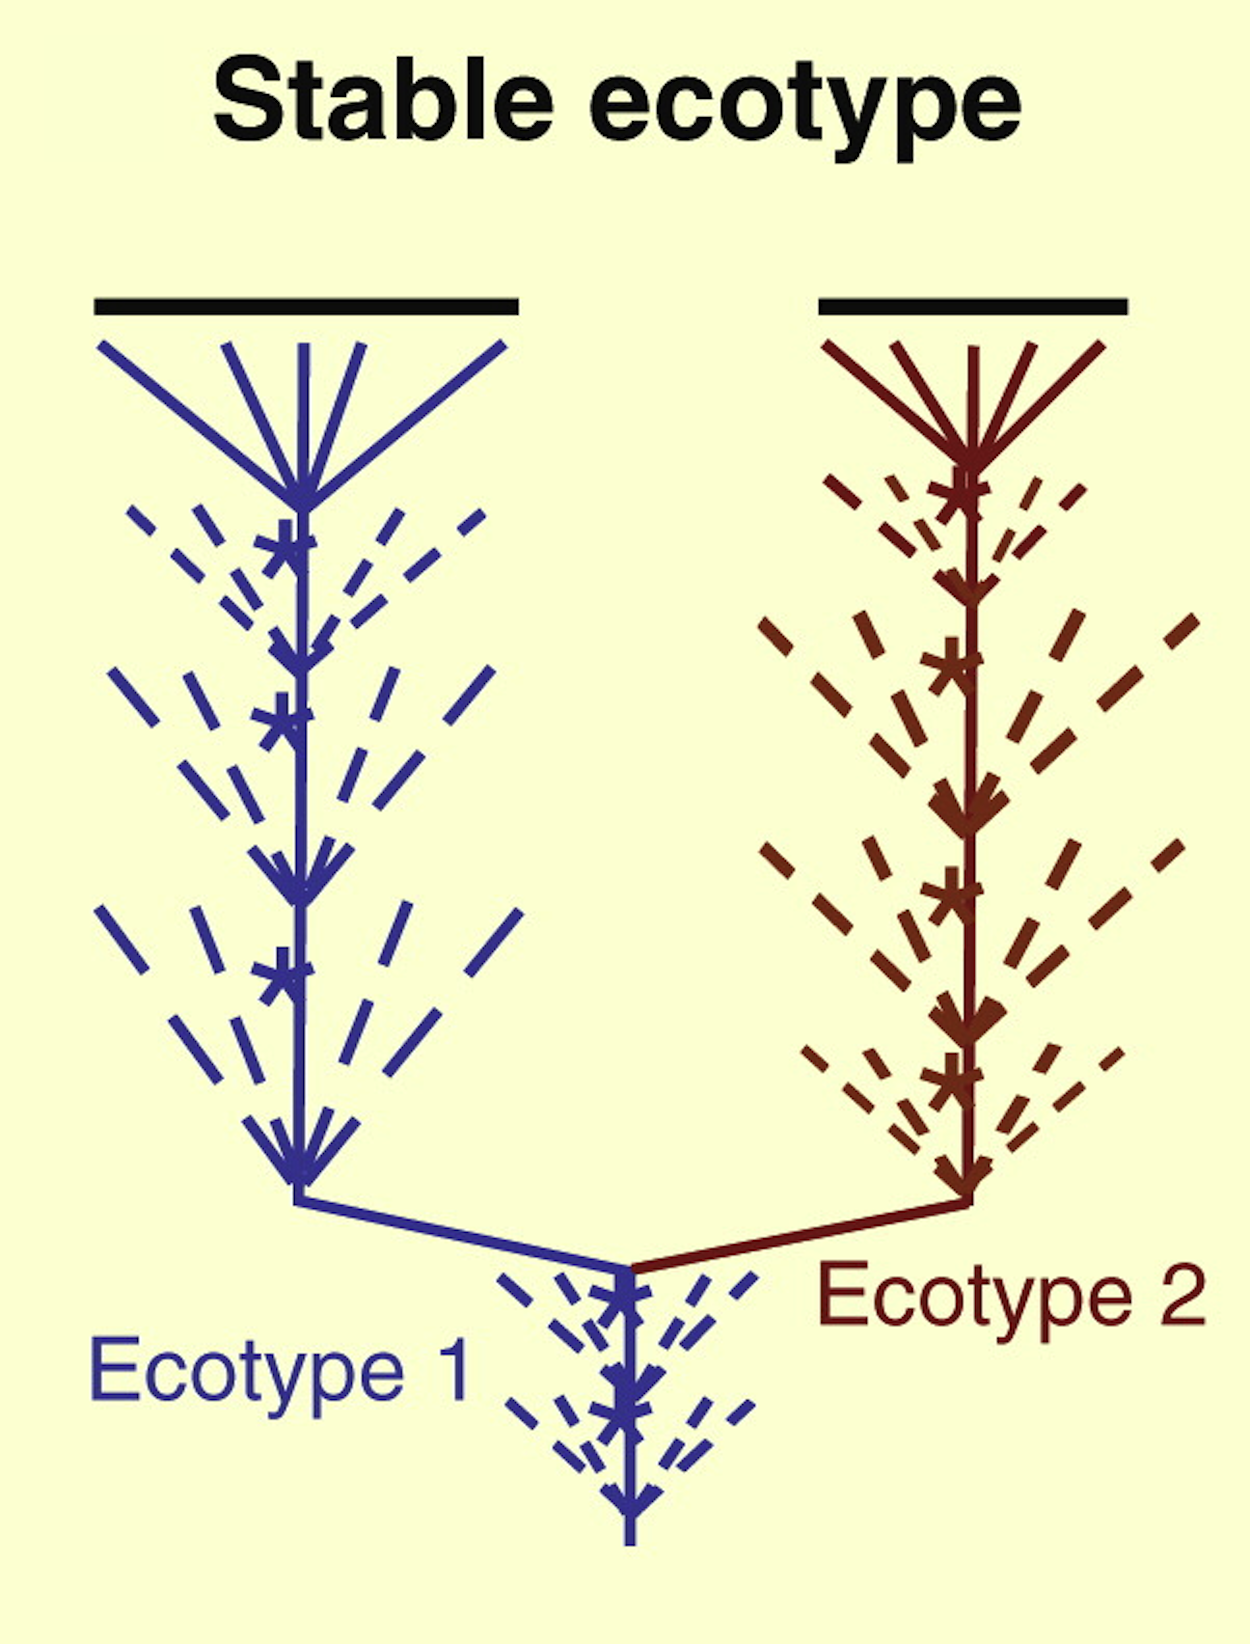
\includegraphics{images/StableTree-CH2}
 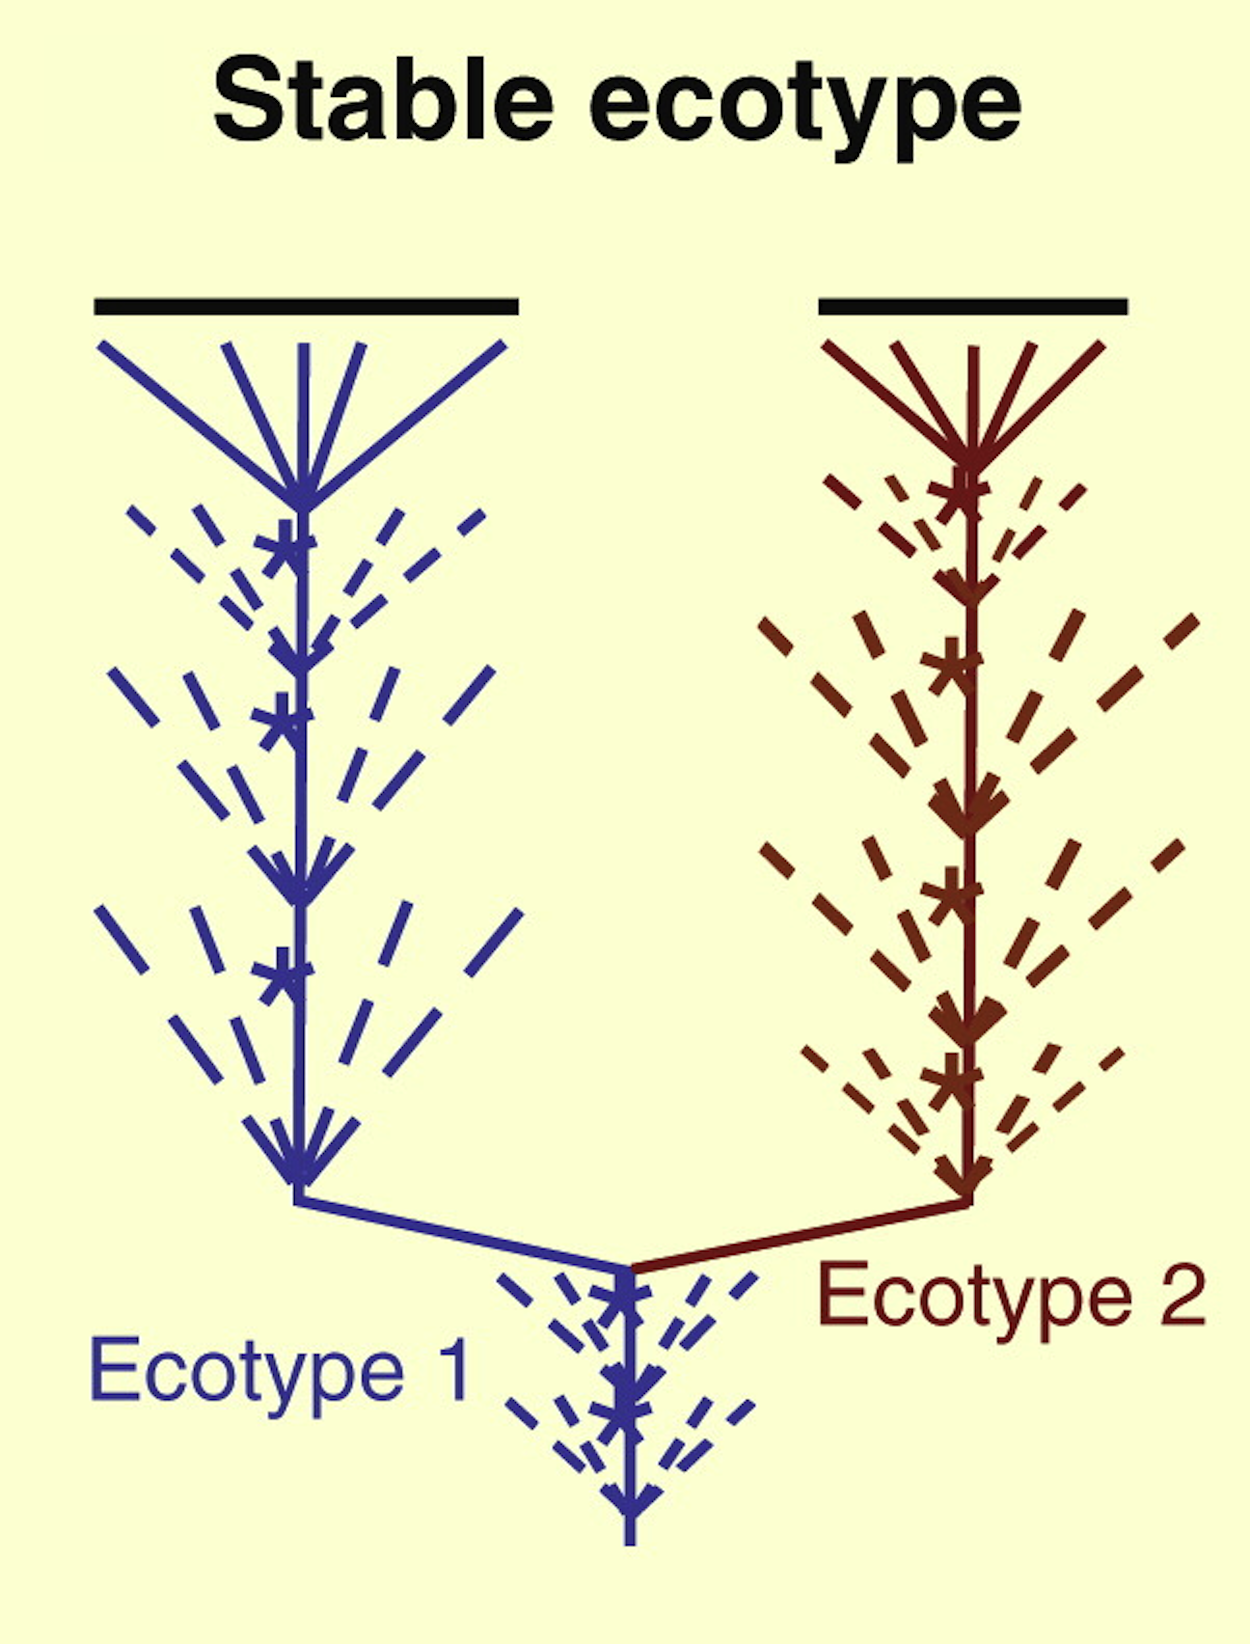
\includegraphics[width=0.5\textwidth]{images/StableTree-CH2}
 %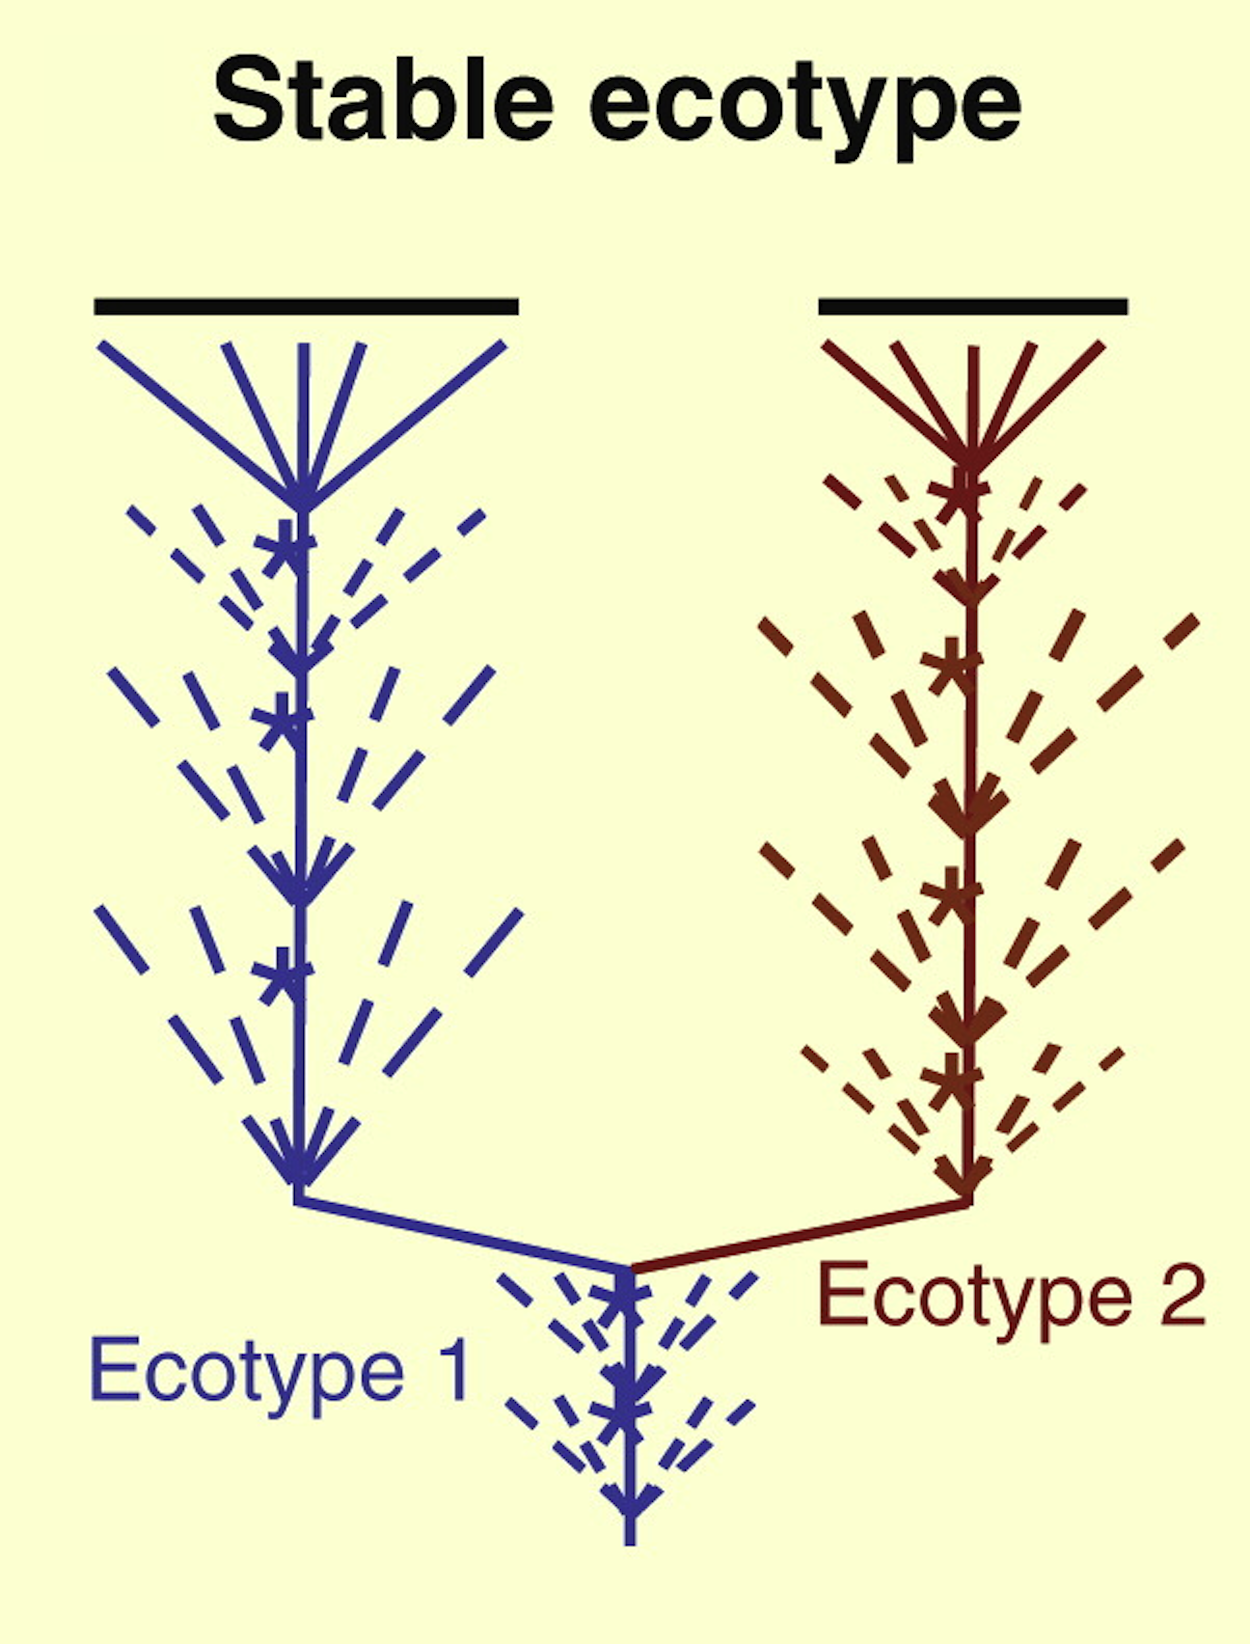
\includegraphics[scale=2.5]{images/StableTree-CH2}
\end{SCfigure}

Utilizing premises established in the Stable Ecotype model we hypothesize a phylogenetic tree similar to the one represented in Figure ~\ref{fig:StableTree}.
Here we can see that ecotype formation is relatively rare, while periodic selection (asterisks) keeps the branches of the tree pruned.
At the point of divergence (where the two solid lines separate into ecotype 1 and 2), organisms from the two separate ecotypes are closely related.
However over time and through various purification events adaptive mutations accumulate.
Notice that the two clades are totally free from each other's periodic selection diversity quashing~\cite{cohan2007systematics}.
This is an important feature of separate ecotypes, because we can later observe the differences acquired from separate evolutionary histories.

Theory and empirical evidence hints that these boundaries correlate to ecological niche, based on empirical studies where environmental samples were collected and statistically correlated to their putative ecotypes~\cite{cohan2007systematics, cohan2006sequence, ward2006cyanobacterial, cohan2006toward}.
To identify the system's fundamental elements takes three steps.
First, observe and characterize the community's evolutionary history.
Second, simulate evolutionary history as hypotheses of various descriptive parameters, resulting in a most likely parametric characterization of observed history.
Finally, demarcate individuals into ecotypes.

\subsection*{Observing and characterizing evolutionary history}
Since the clades are evolving independently we can use the molecular clock characteristic of specific ubiquitous genes.
The gene we choose to measure between organisms must be present throughout.
For this reason ES typically takes in ribosomal gene 16s rRNA, chaperone dnaJ, or gyrase subunit gyrA sequences  as input. Most living organisms have closely related homologues, which is important because we can only demarcate when there exists a homolog.

From the genes we can build a phylogeny that predicts a likely evolutionary history, simply based on sequences.
Because ES only analyzes sequences from non-extinct organisms, the Stable Ecotype model predicts that lineage divergence will be low within the evolutionary history.
And the bacterial diversity sampled is going through various stages of periodic selection purification, thus the end of the phylogeny (temporally closest to the present) will appear frayed (see Figure~\ref{fig:TreeFlare}).

\begin{figure}[h!]
\centering
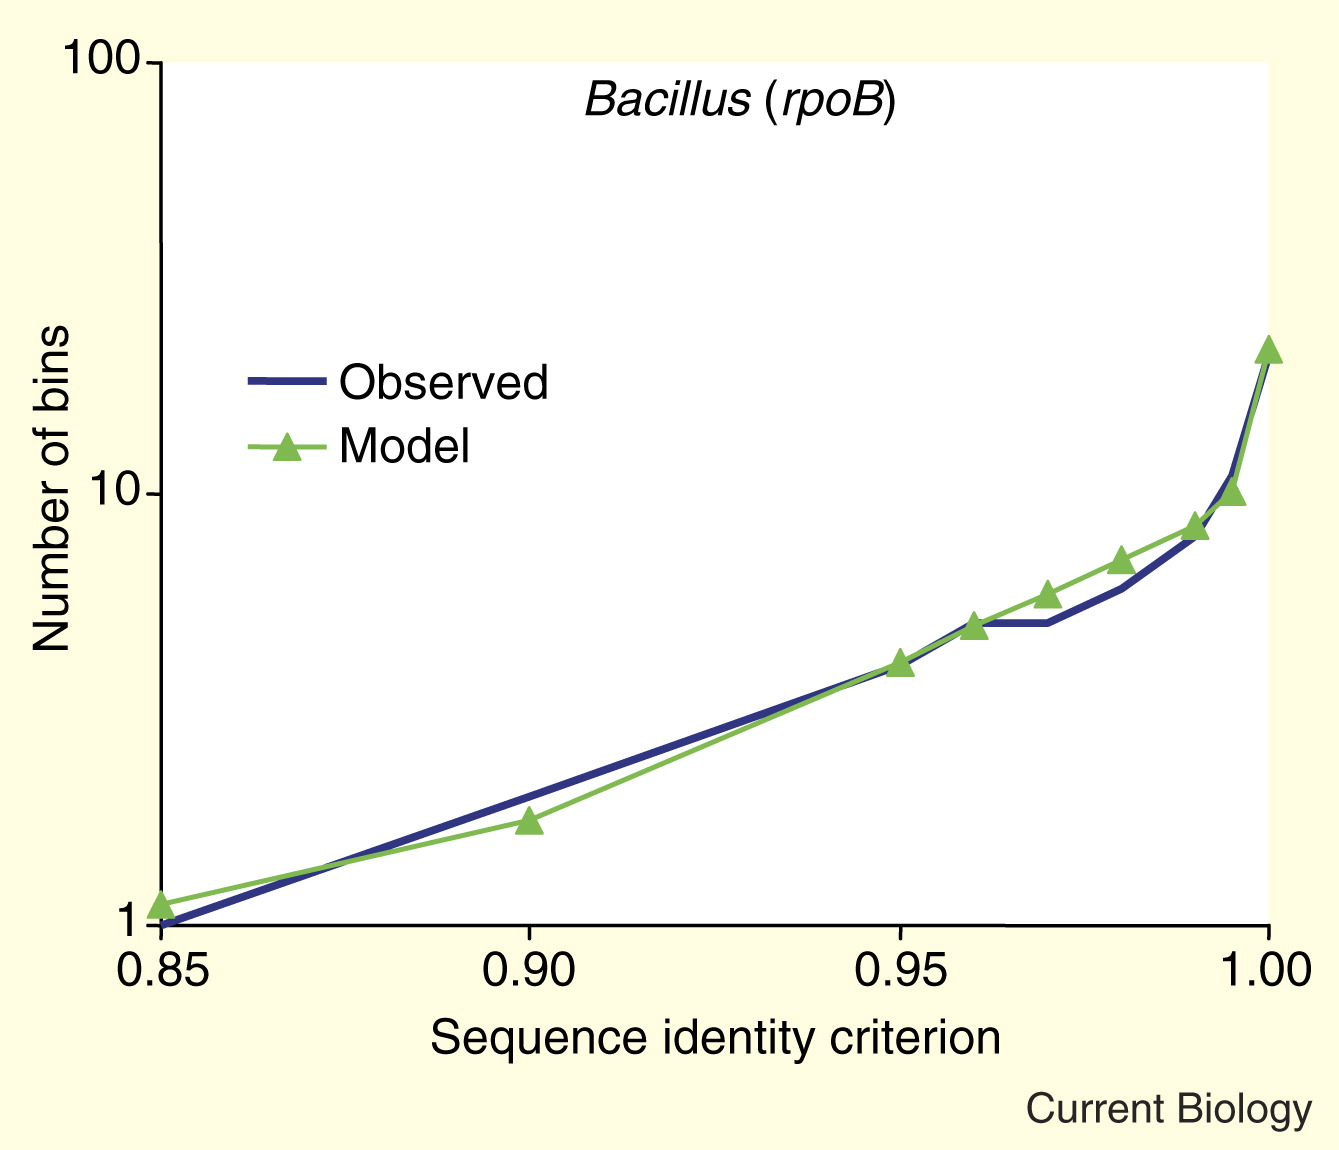
\includegraphics[scale=0.45]{images/TreeFlare-CH2}
\caption[Illustrating the flare at the end of tree due to ecotype diversity.]{Illustrating the flare at the end of tree due to ecotype diversity. Steady accumulation of diversity leads to shallow sequence identity slope, and burst of diversity towards the end of the tree steepen the slope (reprinted from~\protect\cite{fredImage}).}
\label{fig:TreeFlare}
\end{figure}

\subsection*{Simulating evolutionary history}
Starting from observed sequences as separate clusters, ES simulates common divergence, and cohesion events backwards in time, which reduce the number of groups until there is only one cluster representing the common ancestor.
From that ancestor representation with known gene mutation rates, we can simulate sequence diversity through time and generate a collection of gene sequences.
Now this simulated output can be compared to the observed evolutionary history to check for similarity.
By running many (approximately in the millions) simulations, ES develops a maximum likelihood parametric characterization of the observed phylogeny. 

\subsection*{Demarcating ecotypes}
The parametric characterization helps decide how to separate individuals into clusters.
ES progresses temporally from the root of the phylogeny towards the present, analyzing each subtree.
Once there is a certain likelihood that that subtree consists of only one ecotype the demarcation program annotates it as such.


\section{Ecotype Simulation}
%
%   SHOULD WE INCLUDE SAMPLE INPUTS AND OUTPUTS FOR EACH PROGRAM?
%
The current iteration of ES is a GNU General Public Licensed free (as in free speech, not free beer) and open source software written mainly in Fortran 90 with a Java graphical user interface (GUI) that runs on most platforms.
As input it takes a FASTA format file that consists of aligned DNA gene sequences (usually the genes mentioned earlier; concatenated if multiple genes) with an outgroup sequence first, and a corresponding phylogeny, either supplied by the user as a Newick format tree or generated by an optional dependency (Phylip ~\cite{felsenstein1989phylip}) on runtime.
The implementation follows our approach discussed in the previous section, namely, observing evolutionary history, estimating parameter values, and demarcating ecotypes.

\subsection*{Binning}
First the input sequences go through pre-processing to remove nucleotide gaps, and correct for polymerase chain reaction (PCR) error.
Next an $O(n^2)$ space divergence matrix is created using a modified Manhattan (or taxicab) distance metric, where at each base pair position if the two sequences being compared differ in nucleotide we increase the distance by one then divide the total by half the number of base pairs in the sequence.
Distances are estimated according to the Jukes-Cantor model of nucleotide of substitution$$d=-{3\over4} \ln({1-{4\over3}p})$$where $d$ equals distance between two sequences with $p$ substitutions ~\cite{jukes1969evolution}.

The divergence matrix is used to facilitate complete linkage clustering of the sequences, described by the equation $$D(X,Y)= \max_{x\in X, y\in Y} d(x,y)$$ where $d(x,y)$ is the distance between the two elements $x \in X$, and $y \in Y$, and $X$ and $Y$ are two clusters of elements.
The implementation is naive (i.e., $O(n^3)$) and uses a lot of space because of the divergence matrix; there is room for improvement here (I will go into clustering in detail the following chapter). 

\begin{figure}[h!]
 \centering
 \label{fig:Binning}
 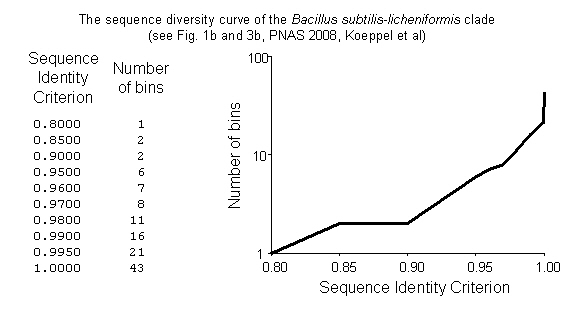
\includegraphics[scale=1.75]{images/Binning-CH2}
 \caption[Sequence identity graph and example output produced by binning.]{An example output of information from the initial binning of sequences from a natural community (reprinted from \protect\cite{koeppel2008identifying}). }
  \label{fig:Binning}
\end{figure}

After binning we observe a sequence identity graph as in Figure \ref{fig:Binning}.
The $x$-axis refers to percent identity between sequences and the $y$-axis the number of bins or clusters.
At low sequence identity criteria there are fewer bins with more sequences in each, and at $1.00$ sequence identity, the number of bins is equal to the number of unique sequences.
A good way to visualize this sequence identity graph is as a linear representation of a phylogeny.
The slope is shallow during lower sequence identities similar to how in a tree we typically see low levels of cladogenesis.
But, as we approach the end of a tree there typically is a fraying of the tips, and in the identity graph there is a corresponding steepening of slope (see Figure \ref{fig:SpeciationGraph}).
Concave departures from an exponential relationship indicate an overabundance of highly divergent lineages (i.e., a very genetically diverse community); convex departures indicate an overabundance of closely related lineages (i.e., a less genetically diverse community~\cite{bohannan2003new}.

We can describe the essence of this graph using four parameters: $npop$, sigma ($\sigma$), omega ($\Omega$), which represent the number of ecotypes, rate of periodic selection (PS), and rate of ecotype formation (EF) respectively.
By finding close approximations of $npop$, $\sigma$, and $\Omega$, we can observe ecotype boundaries within the clade that hypothetically correspond to ecological niche (as stated earlier).

\subsection*{Simulations and likelihood evaluation}
The simulation aspect of ES begins with a process of backwards simulation that stochastically produces a phylogenetic representation of the history of the community.
Think of a node that represents each input organism and sequence from the present time (i.e., number of nodes equals number of input sequences), and the ancestral lineage of these organisms coalesce (due to PS, EF, or D; indicated by gray circles in Figure \ref{fig:SpeciationGraph}) as ES steps backward in time.
Backwards simulation serves as a topological scaffold of history.
Then the forward simulation produces corresponding mutational nucleotide substitution throughout the history of the clade and resulting simulated contemporary organisms are binned, and binning is compared to binning of actual organisms sampled from nature (see Figure~\ref{fig:TreeCompare}).

\begin{figure}[h!]
\centering
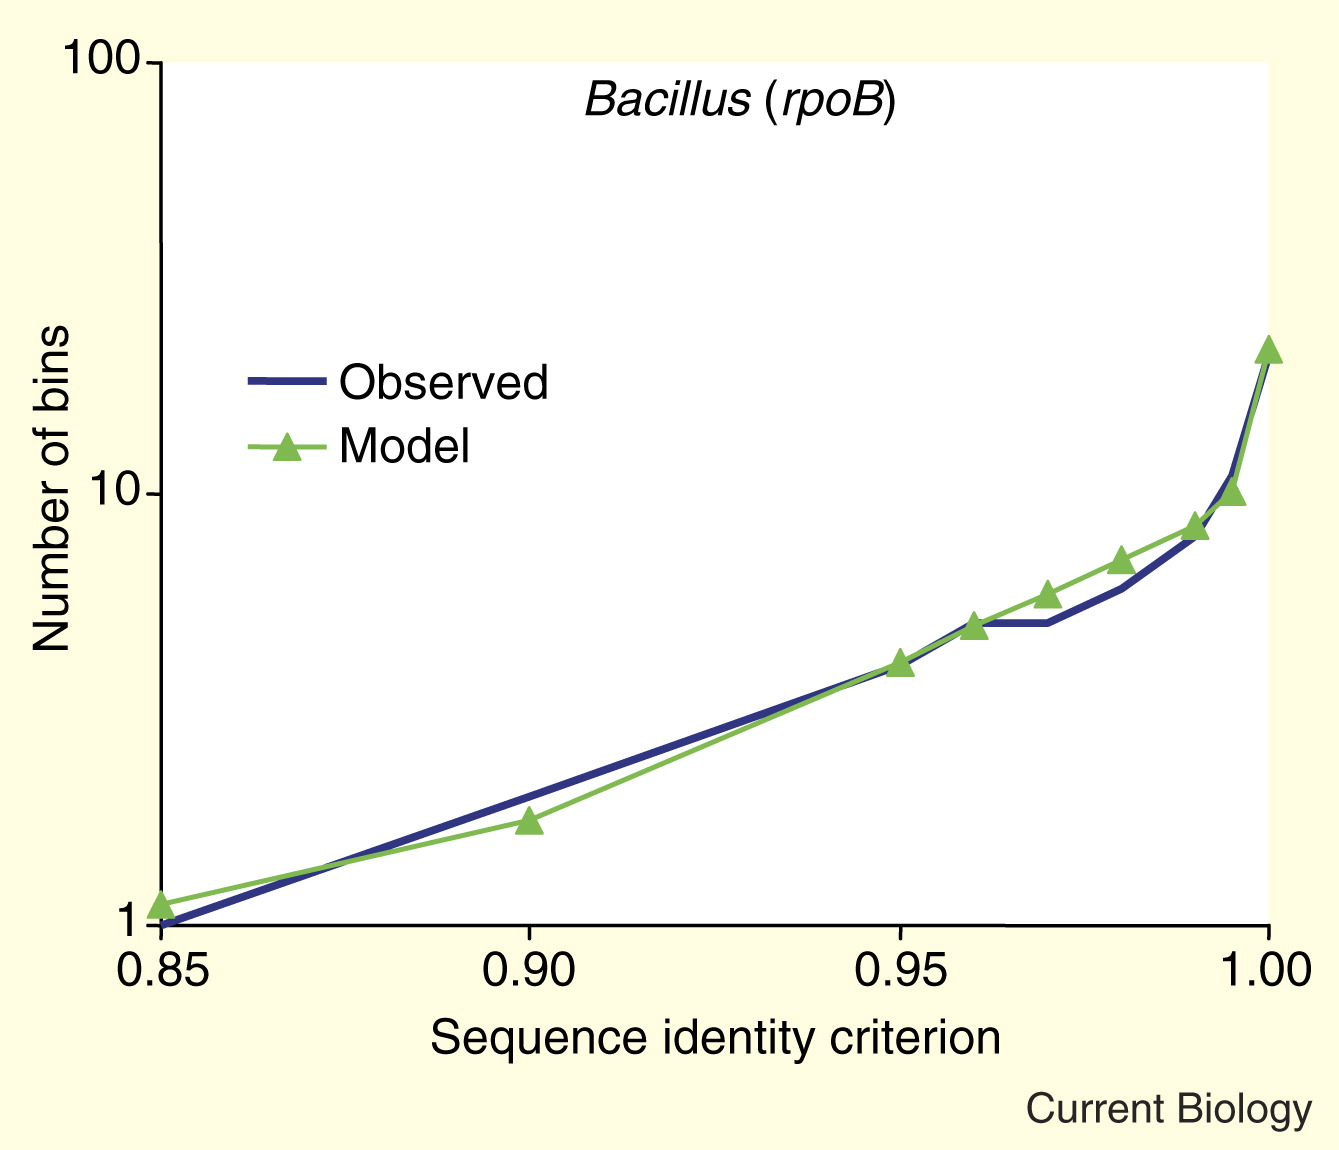
\includegraphics[scale=1.5]{images/TreeCompare-CH2}
\caption[Observed and simulated evolutionary histories.]{Clade sequence diversity, for the \emph{B. subtilis-B. licheniformis} clade, for gene rpoB. A set of 88 sequences from the clade was binned into clusters with different levels of minimum pairwise identity. The log-linear portion of the curve to the left of \textasciitilde0.99 identity indicates a constant net rate of ecotype formation; the flair of diversity to the right of \textasciitilde0.99 indicates the facile sequence diversity within ecotypes~\cite{acinas2004fine}. The ecotype simulation analysis yielded estimates of the parameters for periodic selection rate, net ecotype formation rate, rate of genetic drift, and the number of ecotypes, and the estimated quartet of parameter values generated the ``model'' values shown~\cite{koeppel2008identifying} (reprinted from \protect\cite{cohan2007systematics}).}
\label{fig:TreeCompare}
\end{figure}

Initially a set of $v$ contemporary organisms (representing those sampled from the environment) are randomly distributed according to broken-stick distribution among $n$ ecotypes (in the case of Figure \ref{fig:SpeciationGraph}, $v = 14$ and $n = 3$).
In broken-stick distribution we start with a single giant ecotype then continue to randomly split it up until we have the designated $npop$ ecotypes.
Working backward from the $v$ organisms in the present, the processes of EF, PS, and D occur stochastically in time according to their respective predetermined rates ($\Omega$, $\sigma$, and d).
Each event coalesces one or more lineages into  a single ancestral lineage.
The backward phase of the simulation ends when all of the branches have coalesced into a single node, which represents the most recent common ancestor of the sampled organisms.

\begin{figure}[h!]
%INCLUDE?
%Note that in the backward-looking view of the coalescence formulation, each PS appears as a coalescence event, in which all lineages after the PS coalesce into the survivor of the PS event. Likewise, each D event appears in this backward-looking view as the coalescence of a pair of lineages within an ecotype (e.g., two contemporary lineages coalesce into lineage D1 to reflect the increased representation of lineage D1 after the random loss by drift of lineage D2). 
%Because $\Omega$ is the net rate of EF events, taking into account extinction, we include in the simulation only those EF events resulting in ecotypes that survive into our contemporary sample.

  \centering
   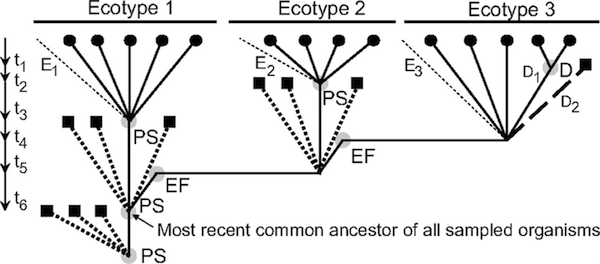
\includegraphics{images/Speciation-CH2}
   \caption[Detailed phylogeny with putative ecotype simulation events.]{A phylogenetic representation of the ecotype simulation algorithm. The algorithm simulates the evolutionary history of the organisms sampled from nature under different values for the net rate of ecotype formation (EF), rates of periodic selection (PS), drift (D), and the number of ecotypes in the sample. It only considers existing individuals (black circles) from non-extinct lineages represented by bold lines. Previously extinguished lineages, due to past PS or D events, are represented by dotted lines and squares (reprinted from \protect\cite{koeppel2008identifying}).}
   \label{fig:SpeciationGraph}
\end{figure}

Forward simulation begins when a sequence the same length as a sampled individual is assigned to the most recent common ancestor.
As time progresses nucleotide substitutions occur stochastically between each pair of nodes (according to the time between the events determining the nodes) in the phylogeny derived from the backward simulation. 
This continues until we reach the contemporary organism nodes, resulting in a matrix of pairwise sequence divergence between $v$ contemporary organisms.

Now ES can conduct the same complete-linkage clustering analysis briefly described in the previous section to illustrate a sequence identity graph, which can be compared to the observed sequence identity graph.
If we place our simulated sequence identity graph line on top of the observed sequence identity graph, at each bin level we can see whether the simulated line matches the observed line within a pre-determined factor (or precision factor).
Success is determined by whether or not these two lines match within this factor of closeness, of which there are six: 5x, 2x, 1.5x, 1.25x, 1.10x, 1.05x.
If the simulation and observed graphs are too far apart (see Figure~\ref{fig:TreeCompare} on page~\pageref{fig:TreeCompare}), ES records the repetition as a failure.
Based on many (i.e., in the hundreds or thousands) replicate runs, each one evaluated for success or failure, we gather information to form a maximum likelihood estimation of $npop$, $\Omega$, $\sigma$, and d (in the future I will not mention drift, since it happens to be so rare). However, how does one decide on different parameter choices to test?

\subsection*{Bruteforce and Hillclimbing}
Utilizing simulations explained in the previous section ES conducts a search for high likelihoods over a multi-dimensional plane (four parameters).
To search as much of that space as possible we lay a grid of points over the landscape of likelihoods where each point is a simulation of many hundreds of repetitions.
By running those tests we begin to observe a rough sketch of hills and valleys of the parameters.
The even distribution of points with a lack of insight is referred to as Bruteforce (see Figure \ref{fig:Flow}A).
The beauty of Bruteforce is that it outputs a range of parameters that contains the global maximum likelihood.
The range of likely parameters is then passed through an optimization program known as Hillclimbing (see Figure \ref{fig:Flow}B), which finds local maximums (i.e., the global maximum within our Bruteforce parameter ranges).

Hillclimbing is a downhill-simplex or Nelder-Mead approach to optimization.
A chosen parameter solution is more thoroughly tested (i.e., with 10,000 replicates), and likelihoods are calculated for the six precision values (i.e., 5x, 2x, etc.).
The program then calculates how long it would have to run to generate 50 success-based runs on the duration of the previous step.
If too much time is required then Hillclimbing runs with a more general precision value.
[I PLAN TO GO INTO MORE DEPTH ON HILLCLIMBING HERE!]
%Describe exact detail of hill climbing optimization. Ask for background paper?


\begin{figure}[h!]
 \centering
 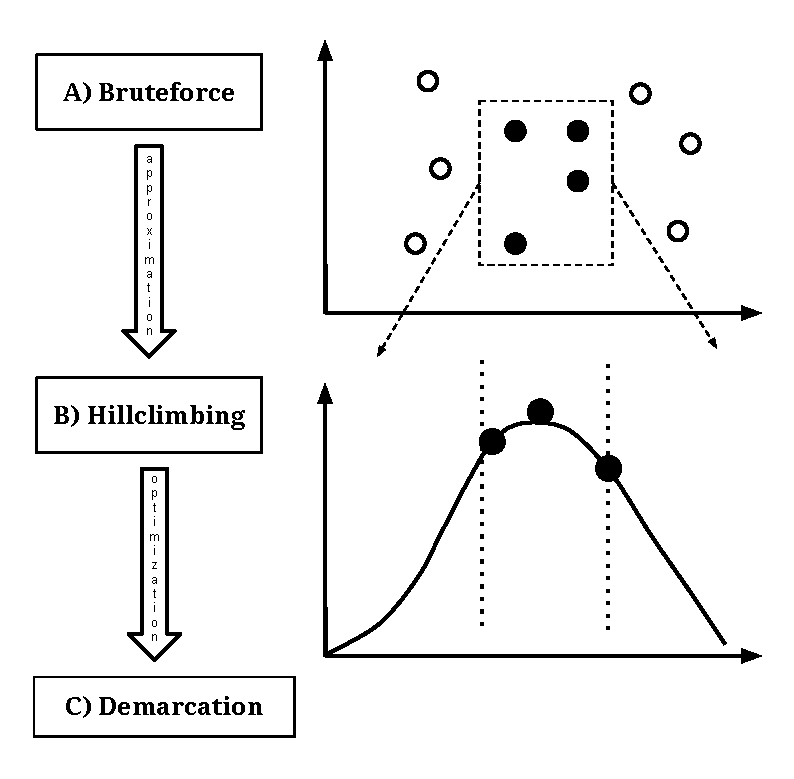
\includegraphics[scale=0.75]{images/ESFlow-CH2.pdf}
 \caption[Ecotype Simulation program flow diagram.]{This is the program call flow of ES. Circles represent simulations, filled are high likelihood successes, while empty are failures. Bruteforce distributes test parameters along the grid, and Hillclimbing figuratively climbs the likelihood hill to find local a maximum (figure created with help from Lingyuan Ke). }
 \label{fig:Flow}
\end{figure}

\subsection*{Demarcation}
With the most likely estimations of $npop$, $\sigma$, and $\Omega$ (remember that we dropped drift since it occurs rarely), we proceed to Demarcation (see Figure \ref{fig:Flow}C).
Demarcation uses the user input phylogeny and the maximum likelihood parameters produced from Hillclimbing optimization (see Figure \ref{fig:Flow}B - C).
ES comes with a manual demarcator, however for my work we used an automatic demarcator that uses a demarcation confidence interval program.

The automatic demarcator starts at the closest common ancestor and recursively runs confidence interval tests for $npop$ on subtrees.
At each level the overall Hillclimbing results are used to run the demarcation confidence interval program which checks parameter likelihoods in a loop that decreases $npop$ by a step value until it is either below 1, beneath a pre-determined likelihood or fails a likelihood ratio test.
The resulting $npop$ from demarcation confidence interval is the 95\% likely lower bound $npop$.
If this $npop$ equals 1 then we demarcate the sequences of the subtree as a single ecotype.
If so, we identify that group of samples as a single ecotype and stop that instance of recursive tree descent.

\section{Ecological Correlation}
Once any algorithm is developed, we must prove its correctness.
In the case of ES, we want to evaluate whether or not predicted demarcations correlate to observed samples.
The Cohan group recommends ecologically checking ES predicted ecotypes, because under various evolutionary models (other than the Stable Ecotype model), a single ecotype may contain multiple sequence clusters \cite{koeppel2008identifying, connor2010ecology}.
Also, we want to demonstrate homogenous ecotypes~\cite{wiedenbeckHGT}, to fully identify fundamental interchangeable units.

This is easier said than done.
Over the past four years the Cohan lab and collaborators have travelled to unique environments around the world gathering samples of bacterial ecosystems and analyzing them with ES, and other demarcation programs.
Following is a short discussion of a few of these studies focused on further insights achieved with ES.

\subsection*{Pyrosequencing analyses of \emph{Synechococcus} ecological species inhabiting the microbial mat of Mushroom Spring, Yellowstone National Park}
%\~cite{pyroEric}
Becraft et. al, used Ti454-barcode high-throughput sequencing to sample more habitat types, obtain deeper sequence coverage per habitat, and sample greater variation within predicted ecological species populations.
ES was then used to demarcate putative ecotypes (PEs) across all high-frequency sequences and microbial mat habitats~\cite{pyroEric}.

They sequenced and analyzed the \emph{psaA} locus because it offers more molecular resolution than 16S rRNA, it exists as a single copy in the genomes of mat \emph{Synechococcus} isolates, it encodes PsaA which is necessary for photosynthesis, and it shows no evidence of recombination~\cite{pyroEric}.
One approach to test for ecological homogenization is to compare temporal patterns of PE-specific gene expression to examine the possibility that PEs respond differently to variations in environmental parameters i.e., testing the response of \emph{Synechococcus} populations to environmental perturbations~\cite{pyroEric}.

Perturbation studies allowed the temporal tracking of genetic diversity within putative ecotypes (PE), allowing us to decide if a PE functioned as a fundamental unit.
They were able to predict and observe homogenous changes in ecotype abundance in response to light and temperature changes~\cite{pyroEric}.

Thus, through \emph{psaA} analysis they showed that the most abundant PEs predicted by ES are ecologically distinct, and by studying environmental perturbations they provided evidence hinting at ecological homogeneity; the two requirements for identifying an ecotype.

%\subsection*{Radio Facility Wash Paper}
\subsection*{Ecology of Speciation in the Genus \emph{Bacillus}}
%The ecology of speciation in Bacillus connor2010ecology
Connor, et. al., sampled bacteria from the \emph{Bacillus subtilis-Bacillus licheniformis} clade from sites differing in solar exposure and soil texture within a Death Valley canyon.
Within the sample clade they hypothesized ecotype demarcations based on DNA sequence diversity through the clade's evolutionary history analysis with ES.
Ecotypes demarcated were found to be significantly different in their associations with solar exposure and soil texture~\cite{connor2010ecology}.
In the study they were attempting to provide a new protocol for describing and discovering the ecotypes of a microbial clade.
However, they were careful to show that groups predicted by ES correlate to environmental characteristics; one such significant example was the solar exposure, clearly connecting species and an ecological niche.

The recognized species and subspecies of the sampled clade were found to be nearly identical to the ecotypes demarcated by ES.
Nevertheless, the taxa recognized do not appear to encompass the full ecological diversity of the clade~\cite{connor2010ecology}.
ES predicted putative ecotypes not recognized as species or subspecies in one case they identified the ecological dimensions of divergence, suggesting that the \emph{B. subtilis-B. licheniformis} clade is replete with newly divergent ecotypes~\cite{connor2010ecology}. [REWRITE!]

%replaced with paper that is just coming out...
%\subsection*{Yellowstone hot spring paper}
%\subsection*{Fine-Scale Distribution Patterns of \emph{Synechococcus} Ecological Diversity in Microbial Mats of Mushroom Spring, Yellowstone National Park}
%Fine-scale distribution patterns of Synechococcus becraft2011fine
%Scientists sampled the \emph{psaA} (which encodes a photosynthetic reaction center protein) locus from the genus \emph{Synechococcus} and studied distribution variants at 1$^\circ$C intervals along the effluent flow channel at 80-$\mu$m vertical-depth intervals throughout the upper photic layer of the microbial mat~\cite{becraft2011fine}.
%Once again a microbial community is sampled for a common DNA sequence.
%In this case the thinking is that the various layers of bacterial organisms differ in photosynthetic specialization, thus the choice of \emph{psaA}, which offers more molecular resolution.
%However, since we use a molecular approach that measures a single gene carefully, even correlation between ecological niche and ecotype provides evidence for accurate demarcation.
%
%The microbial mats at the 60 and 63$^\circ$C sites both exhibited steep gradients of O$_2$, pH, and irradience with depth, leading to microenvironmental niche opportunities in the mats.
%The group used denaturing gradient gel electrophoresis (DGGE) to track the distributions of PEs predicted by ES.

%\subsection*{Death Valley Salinity}
\subsection*{Diversity of Bacteria and Archaea in hypersaline sediment from Death Valley National Park, California}
%Death Valley salinity kim2012diversity
The objective of this study was to analyze the evolutionary history of microorganisms from the domains Bacteria and Archaea in hypersaline sediment from Death Valley National Park~\cite{kim2012diversity}. 
They looked at a region of the 16s rRNA gene.
A set of 130 \emph{Bacillus} isolates formed a subclass of the \emph{B. subtilis-B. licheniformis} clade, forming four newly discovered clades (see Figure \ref{fig:DeathES}) that were each identified as an ecotype by ES. Evidence for ecological divergence among the putative ecotypes is provided by the significant tendencies of these groups to be isolated from different media~\cite{kim2012diversity}.

Here we see another example of exploring microbial diversity through molecular means.
But the list of possible applications is endless.
In fact we are at the point where increasing the input size is quite important so we can attempt to grasp a more complete picture of bacterial diversity (which as we have already established is probably in the millions~\cite{cohan2008origins}).

\begin{figure}[h!]
\centering
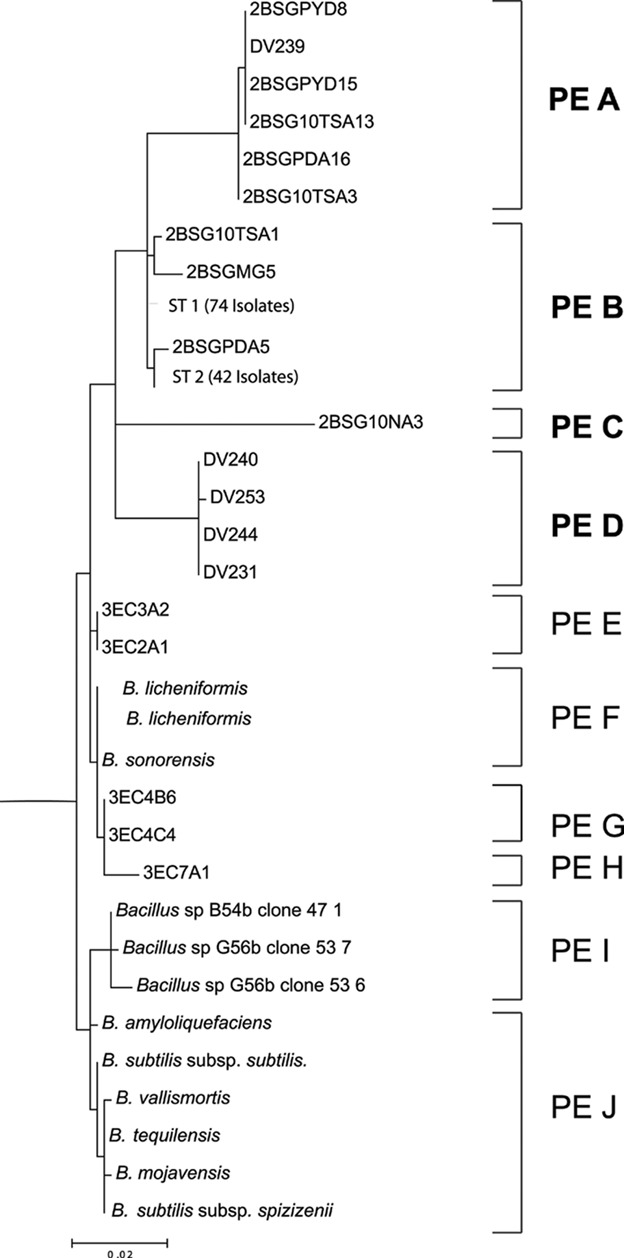
\includegraphics[scale=0.45]{images/DeathValleyES-CH2}
\caption[Example ES analysis of 16s rRNA sequences of isolates from the \emph{B. subtilis-B.licheniformis} clade.]{Maximum likelihood phylogeny and Ecotype Simulation analysis of 16S rRNA sequences of isolates from the \emph{B. subtilis-B. licheniformis} clade. All isolates of this study from this clade were members of a previously unknown subclade that Ecotype Simulation demarcated into Putative Ecotypes A-D (in bold); previously studied organisms from other environments were members of Putative Ecotypes E-J. The tree is rooted by \emph{B. halodurans} strain C-125 (reprinted from\protect\cite{kim2012diversity}).}
\label{fig:DeathES}
\end{figure}

\section{Chapter Summary}
Here we introduced the ecotype model of bacterial species, which defines species as a bacterial cluster with genetic diversity limited by a cohesive force.
Then we explored various possible factors affecting evolutionary history in the Stable Ecotype model of bacterial speciation, which provide the grounding in theory necessary to develop an algorithm for demarcation.
Specifically through the use of periodic selection, drift purification, and ecotype formation events.

After generally discussing the algorithm behind ES, we got our hands dirty and described each important step of ES in detail, including Binning, simulations, Bruteforce, and Hillclimbing (see Figure~\ref{fig:Flow}).
Finally, I briefly surveyed a few studies where we attempted and succeeded in displaying the statistical significance of ES bacterial species demarcation.

In the following section I will discuss the work we have done recently in improving ES.




